\subsection{Smoothed Particle Hydrodynamics}
Smoothed Particle Hydrodynamics is a numerical simulation method first introduced by \cite{Monaghan_1977} in 1977. It is a Lagrangian particle method and as such often used when the geometry of the underlying problem makes it difficult to apply Eulerian grid-based methods like finite difference schemes. Although SPH is most often used to model liquids, it is possible to add physical models for solids as well.

A SPH simulation is composed of many individual SPH particles. Each particle moves through space with a velocity $\vec{v}$ and a mass m. In contrast to particle methods used for N-body simulations or molecular dynamics, SPH particles carry information about continuous variables such as the density $\rho$ or energy e. The particles only act as computational points at which equations from hydrodynamics/continuum mechanics such as the Euler or Navier-Stokes Equations are evaluated. Solving such equations comes down to converting partial differential equations to a system of first order ordinary differential equations in time.

\begin{equation} \label{eq:ode}
    \frac{d\vec{y}}{dt} = f(t, \vec{y}(t), A_1, ..., A_n)
\end{equation}

In equation \ref{eq:ode} $\vec{y}$ is a vector of quantities to be projected forward in time and $A_1$ through $A_n$ are quantities that are calculated at every step. Once $A_1$ through $A_n$ are known for every particle and the right hand side of quation \ref{eq:ode} can be evaluated, standard integrators such as Runge-Kutta or Predictor-Corrector methods are used to update $\vec{y}$.

To calculate a quantity A at a particle location, SPH uses a weighted average of A over all particles in the neighborhood:

\begin{equation}
    A(\vec{r}\,) \approx \int A(\vec{r}\,') W(\vec{r} - \vec{r}\,', h) \mathrm d\vec{r}\,'
\end{equation}

The kernel function $W(|\vec{r} - \vec{r'}|$, h) at the particle location $\vec{r}$ depends upon the distance to the other particles and a specific length h called the smoothing length. Most kernels used today have compact support within a radius of h. To ensure normalization of the kernel

\begin{equation} \label{eq:kernel_normalization}
    \int W(\vec{r} - \vec{r}\,', h)\mathrm d\vec{r}\,' = 1
\end{equation}

in the practial case of a finite number of particles, the density is added to
\begin{equation}
    {\displaystyle A_{S}({\vec {r}}\,)=\lim \limits _{h\rightarrow \infty }\int {\frac {A({\vec {r}}\,')}{\rho ({\vec {r}}\,')}}W({\vec {r}}-{\vec {r}}\,',h)\rho ({\vec {r}}\,')\mathrm {d} {\vec {r}}\,'\propto \sum \limits _{b=1}^{N}m_{b}{\frac {A_{b}}{\rho _{b}}}W({\vec {r}}-{\vec {r}}\,',h)=A_{b}}
\end{equation}




\begin{equation}
    \int_{}^{} W(|\vec{r} - \vec{r'}|, h)dr' = 0
\end{equation}


Figure \ref{fig:smoothing_kernel} illustrates

\begin{figure}[H]
    \centering
    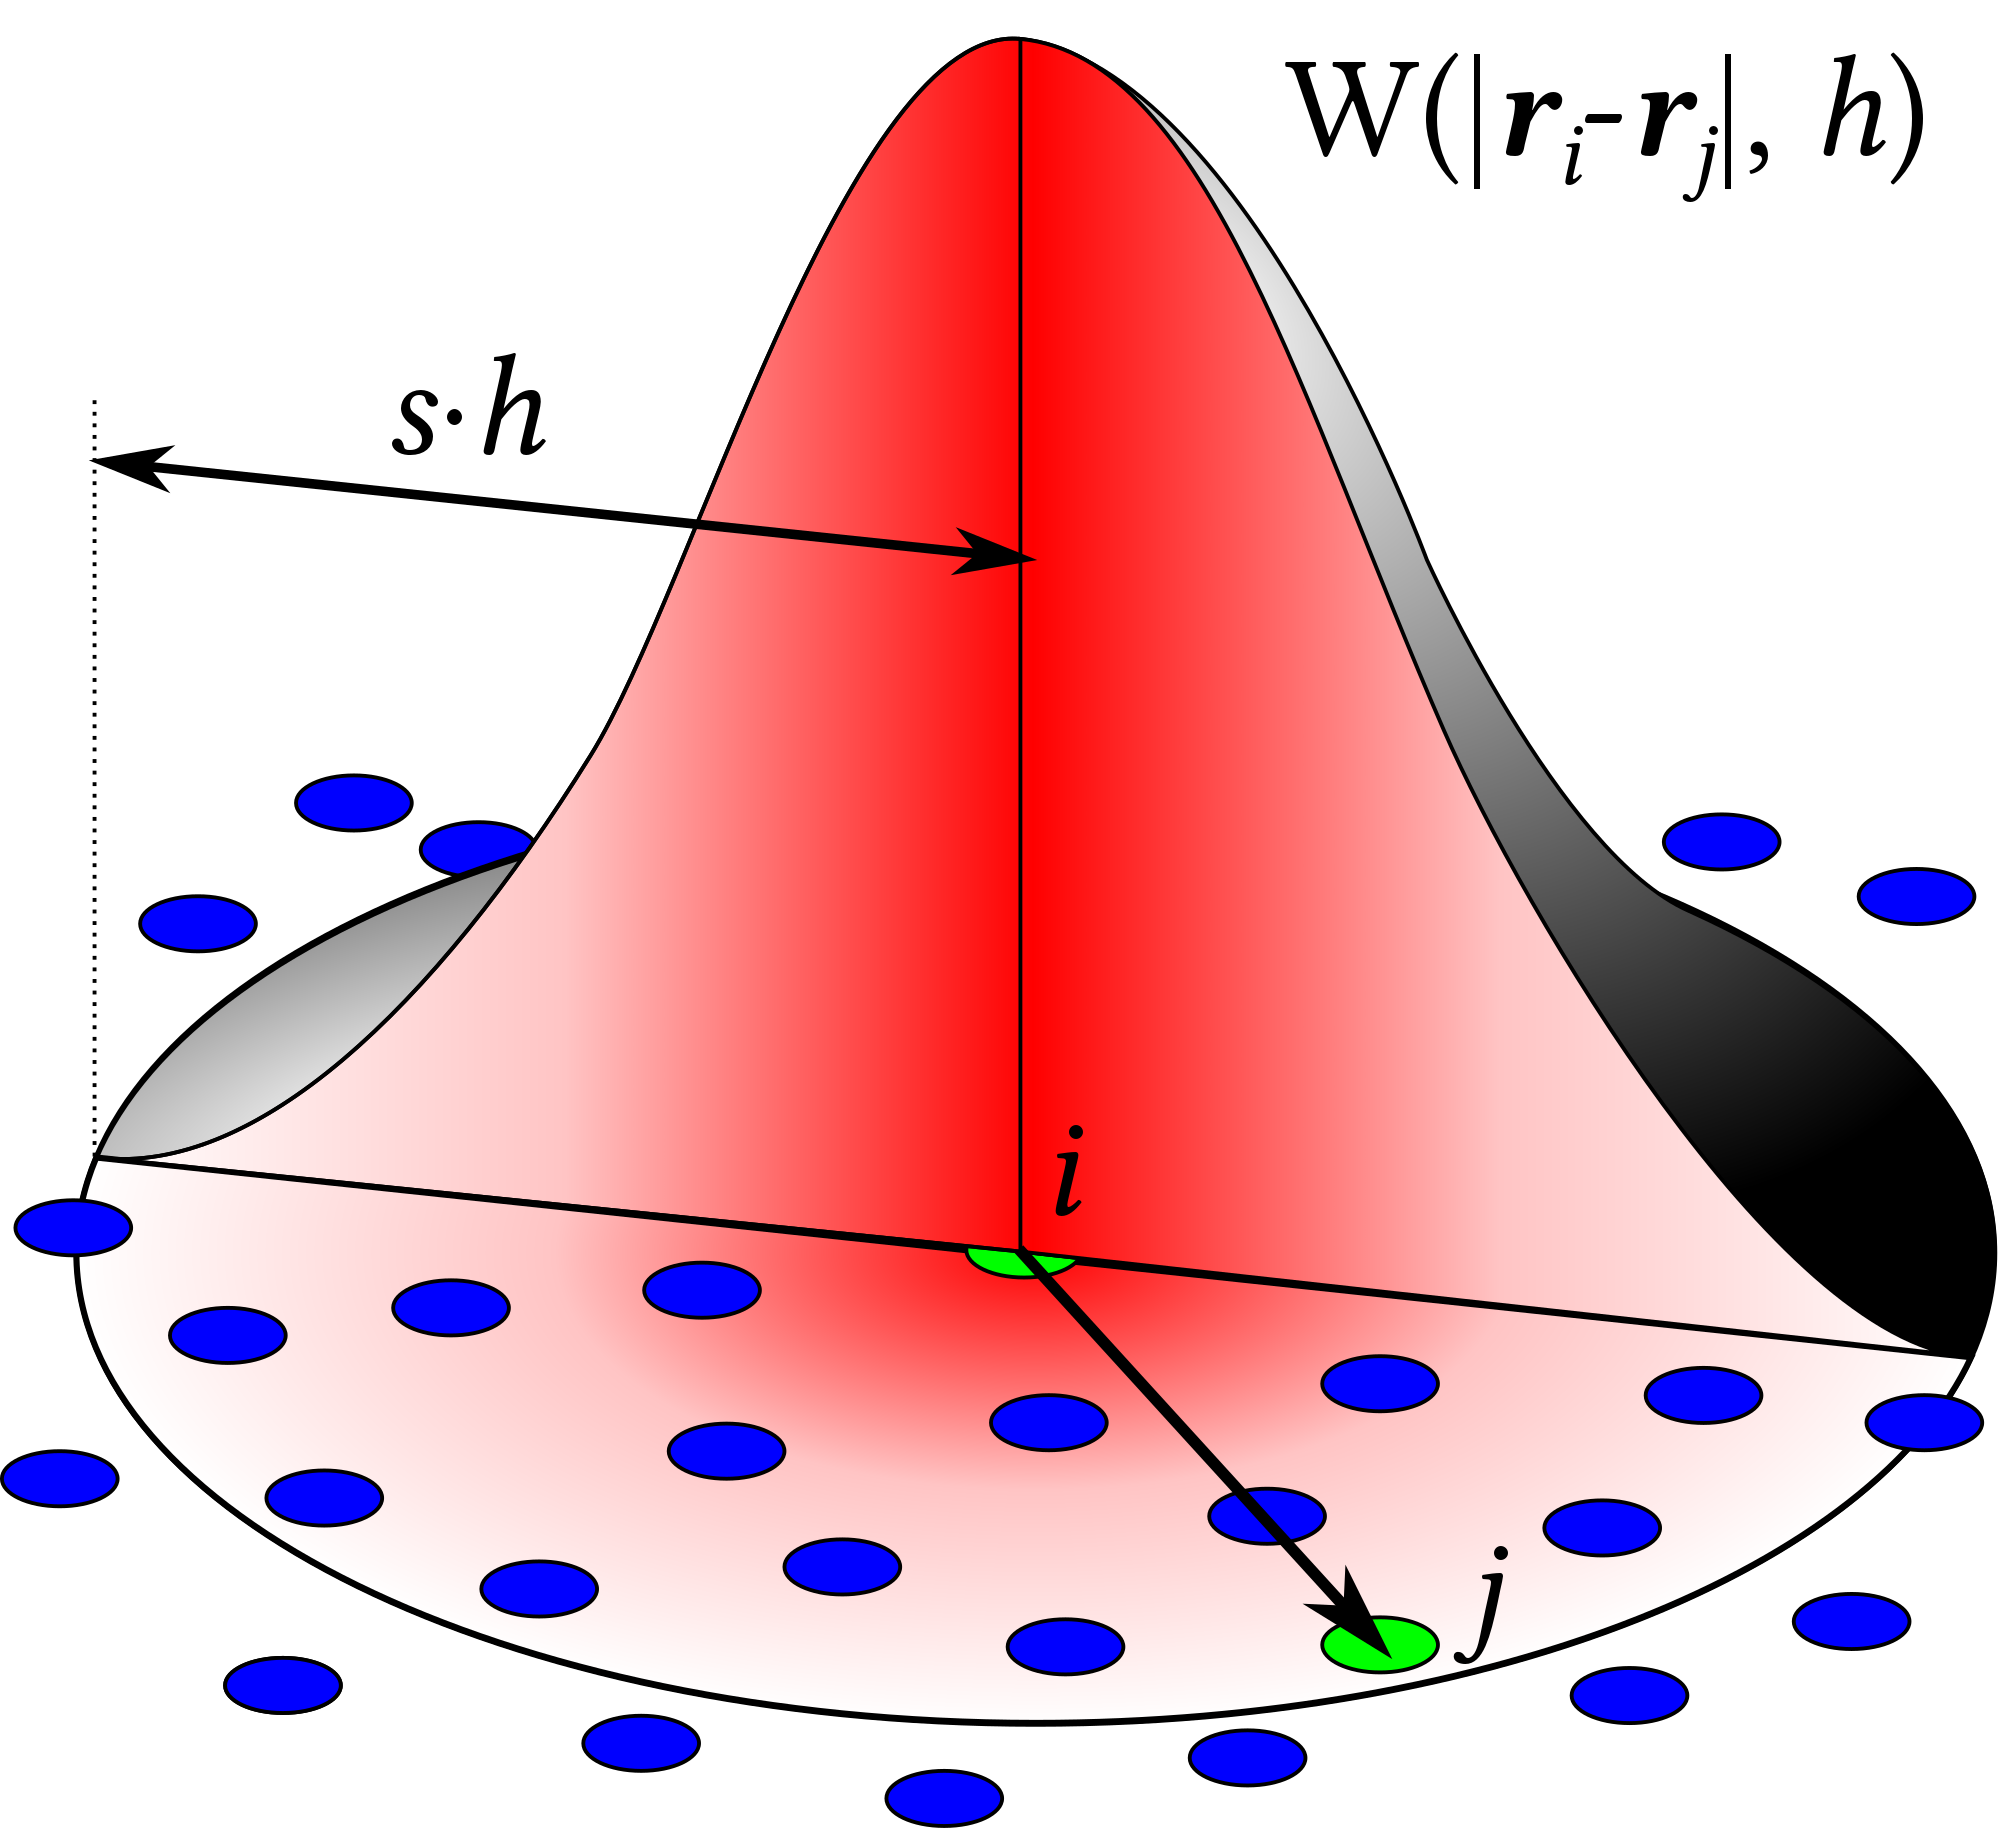
\includegraphics[width=0.5\textwidth]{smoothing_kernel.png}
    \caption{Kernel function \cite{wiki:smoothing_kernel}}
    \label{fig:smoothing_kernel}
\end{figure}

\subsection{Miluphcuda SPH code}
Miluphcuda is a GPU accelerated smoothed particle hydrodynamics code that has been developed over several years at the University of Tuebingen by Christoph Schaefer and others. Its general use is well documented in \cite{Schaefer_2016}. Since the publication of the paper additional models for porosity and strength have been implemented.


\subsubsection{Equation of State}
The Tillotson equation of state \cite{Tillotson_1962}


\subsubsection{Porosity model}
There are different ways in which porosity can be modeled depending on the pore size. Depending on the simulation, macro porosity with pore sizes above the resolution of the simulation can be accounted for in the initial conditions. This however becomes impossible for granular material with sub-resolution sized grains and pores.

Microporosity models porosity as an additional material property and can be applied independently of the resolution.


In these simulations, a microporosity p-$\alpha$ model as outlined in \cite{Jutzi_2008} is used. The distention $\alpha \in [1,\inf)$ relates the current density $\rho$ to the solid density $\rho_s$ which is reached if the material is fully compressed. For a non-porous material $\alpha$ equals one.

\begin{equation}
    \alpha \equiv \frac{\rho_s}{\rho}
\end{equation}

Often the porosity $\phi$ is used instead of the distention $\alpha$. They relate by

\begin{equation}
    \phi = 1 - \frac{1}{\alpha}
\end{equation}

Quadratic crush curve
\subsubsection{Strength model}

\subsubsection{Time Integration}